\section{Results}
If not stated differently the simulations use parameters as given in the table below:
\begin{table}[H]
    \centering
    \begin{tabular}{r|l}
        $N$ & $10^{5}$\\
        $D$ & $0,02$\\
        $R_s$ & $1$ \\
        $R_d$ & $10$ \\
        ${\rm d}t$ & $10^{-3}$
    \end{tabular}
    \caption{Default simulation parameters}
    \label{tab:Parameters}
\end{table}
The following figures show results of simulations using the model explained before. First we examine the dependence of the reaction rate on the diffusion constant. Therefore the simulation results are compared to the steady state analytic solution derived from \eqref{ideal reaction rate}:
\begin{align}
    K &= 4 \pi R_s D \rho_o \\
    \rho_o &= N \left\{ \int_{R_s}^{R_d} \left( 1 - \frac{R_s}{r} \right) {\rm d} r \right\}^{-1}
    \label{Steady_state_rate}
\end{align}
\begin{figure}[H]
    \centering
    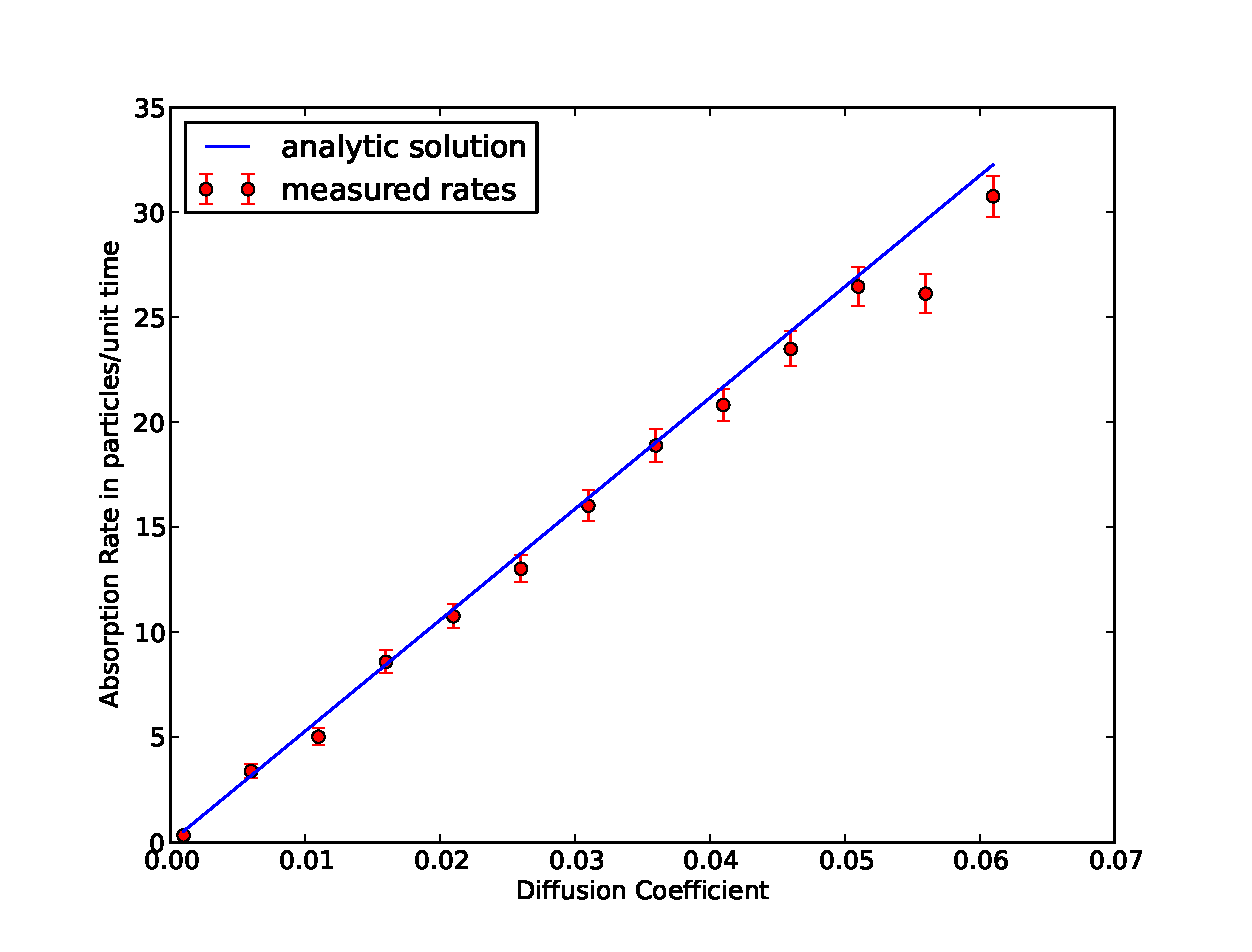
\includegraphics[width=.9 \textwidth, keepaspectratio]{Kabs.eps}
    \caption{Reaction rates vs. Diffusion coefficient - Analytic solution and measured results}
    \label{fig:Kabs_D}
\end{figure}
The preceeding figure shows the results for several simulation runs with different diffusion coefficient. It is obvious that the simulation results show the correct linear behaviour for the reaction rate but have a systematic error of about $5 - 10 \%$. To give a better impression of the relational dependence the following plot shows relative quantities for the results:
\begin{figure}[H]
    \centering
    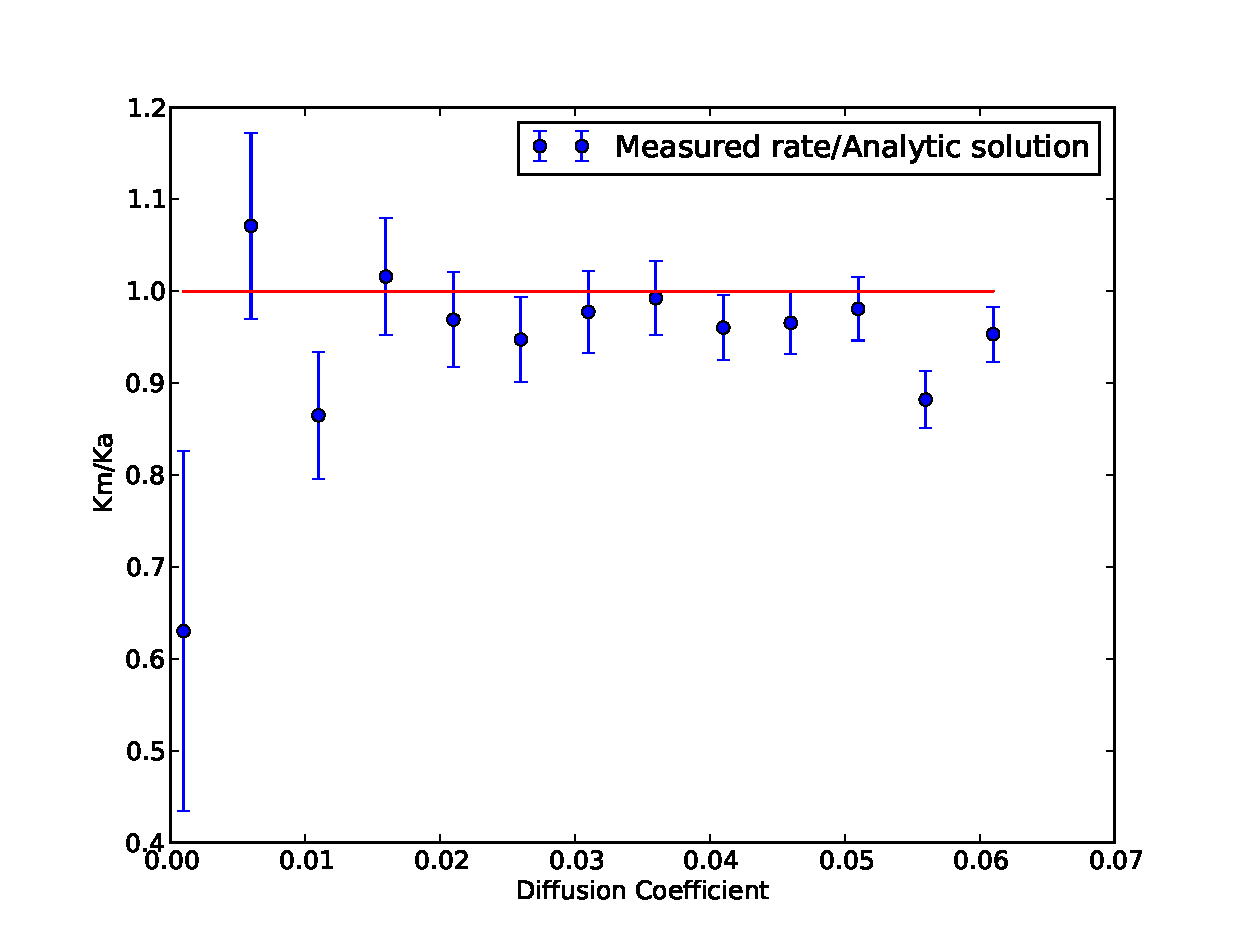
\includegraphics[width = .9 \textwidth, keepaspectratio]{Krel.eps}
    \caption{Relative quantities for Reaction rates}
    \label{fig:Krel_d}
\end{figure}
